\documentclass{article}

\usepackage{graphicx}
\usepackage{tikz}
\usepackage{tikzsymbols}
\usetikzlibrary{calc,patterns,shapes.geometric}
\pagestyle{empty}
\usepackage[margin=0pt]{geometry}
\geometry{papersize={14in,12in}}

\def\centerarc[#1](#2)(#3:#4:#5){\draw[#1] ($(#2)+({#5*cos(#3)},{#5*sin(#3)})$) arc (#3:#4:#5);}

\begin{document}
	\begin{figure}
		\centering
		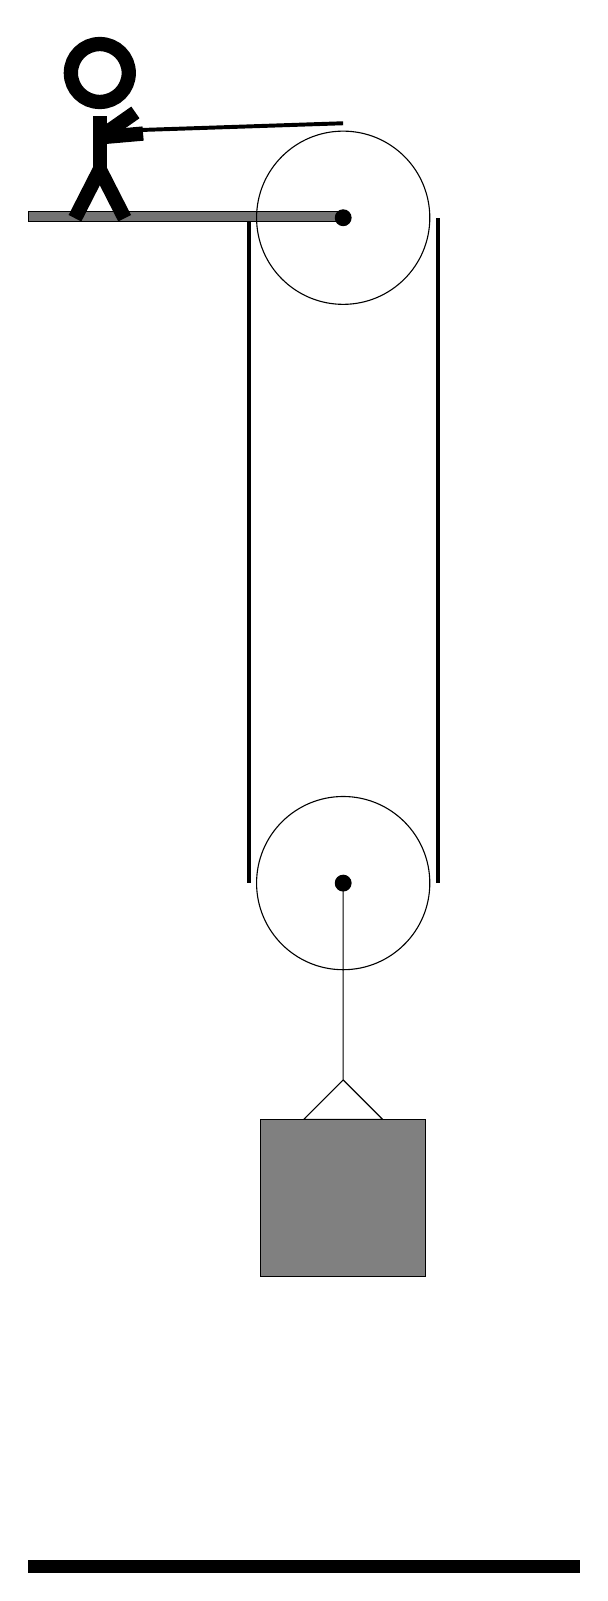
\begin{tikzpicture}
			%%%%% START %%%%%
			\draw[fill=black!55] (-2, 14) rectangle (2, 14.125);
			
			\draw (2, 5.6) circle (1.1);
			\draw[fill=black] (2, 5.6) circle (0.1);
			
			\draw (2, 14.05) circle (1.1);
			\draw[fill=black] (2, 14.05) circle (0.1);
			
			\draw (2, 5.6) -- (2, 3.1) -- (1.5, 2.6) -- (2.5, 2.6) -- (2, 3.1);
			\draw[fill=black!50] (0.95, 2.6) rectangle (3.05, 0.6);
			
			\draw[line width=0.5mm] (0.8, 14) -- (0.8, 5.6);
			\centerarc[line width=0.5mm](2, 5.6)(180:360:1.2000000000000002);
			\draw[line width=0.5mm](3.2, 5.6) -- (3.2, 14.05);
			\centerarc[line width=0.5mm](2, 14.05)(0:90:1.2000000000000002);
			\draw[line width=0.5mm](2, 15.25) -- (-1, 15.15);
			
			\node at (-1, 15.15) {\Strichmaxerl[10][-175][35]};
			
			\draw[fill=black] (-2, -3) rectangle (5, -3.15);
			%%%%% END %%%%%
		\end{tikzpicture}
	\end{figure}	
\end{document}